
\documentclass[12pt]{article}
\usepackage{tikz}
\usetikzlibrary{positioning,arrows,patterns}
\begin{document}
\pagestyle{empty}


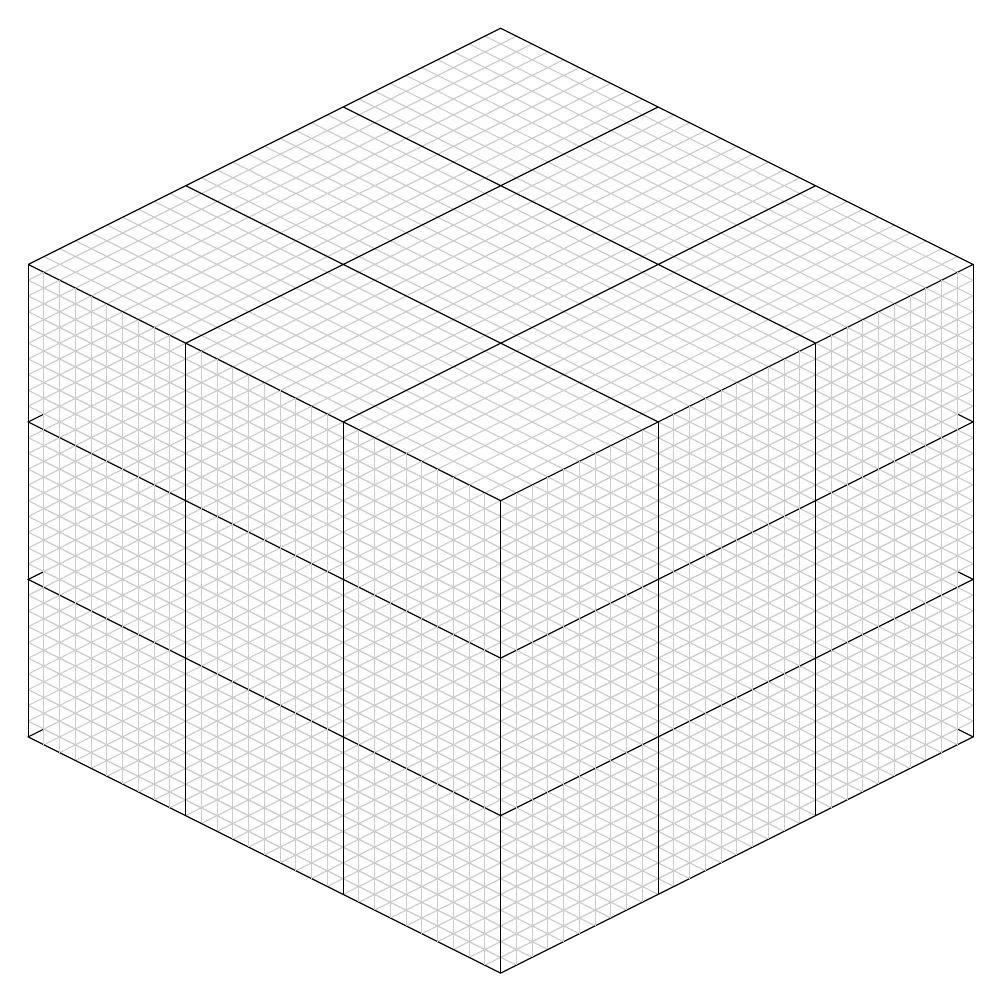
\begin{tikzpicture}[scale=2,every node/.style={minimum size=1cm},on grid]

	% Bottom of cube
	\begin{scope}[
			yshift=0,every node/.append style={
			yslant=0.5,xslant=-1},yslant=0.5,xslant=-1
		]
		\fill[white,fill opacity=0.9] (0,0) rectangle (3,3);
		\draw[step=1mm, black!20,thin] (0,0) grid (3,3);
		\draw[step=10mm, black] (0,0) rectangle (3,3);
	\end{scope}

	% Layers over it
	\foreach \y in {1,2,...,10} {
		\begin{scope}[
				yshift=\y mm,every node/.append style={
				yslant=0.5,xslant=-1},yslant=0.5,xslant=-1
			]
			\fill[white,fill opacity=0.9] (0,0) rectangle (3,3);
			\draw[step=1mm, black!20,thin] (0,0) grid (3,3); 
		\end{scope}
	}

	% Division
	\begin{scope}[
			yshift=10mm,every node/.append style={
			yslant=0.5,xslant=-1},yslant=0.5,xslant=-1
		]
		\draw[step=10mm, black] (0,0) rectangle (3,3);
	\end{scope}


	% More layers
	\foreach \y in {11,12,...,19} {
		\begin{scope}[
				yshift=\y mm,every node/.append style={
				yslant=0.5,xslant=-1},yslant=0.5,xslant=-1
			]
			\fill[white,fill opacity=0.9] (0,0) rectangle (3,3);
			\draw[step=1mm, black!20,thin] (0,0) grid (3,3); 
		\end{scope}
	}

	% Mid layer
	\begin{scope}[
			yshift=20mm,every node/.append style={
			yslant=0.5,xslant=-1},yslant=0.5,xslant=-1
		]
		\draw[step=10mm, black] (0,0) rectangle (3,3);
	\end{scope}

	% More layers
	\foreach \y in {21,22,...,29} {
		\begin{scope}[
				yshift=\y mm,every node/.append style={
				yslant=0.5,xslant=-1},yslant=0.5,xslant=-1
			]
			\fill[white,fill opacity=0.9] (0,0) rectangle (3,3);
			\draw[step=1mm, black!20,thin] (0,0) grid (3,3); 
		\end{scope}
	}

	% Top layer
	\begin{scope}[
			yshift=30mm,every node/.append style={
			yslant=0.5,xslant=-1},yslant=0.5,xslant=-1
		]
		\fill[white,fill opacity=0.9] (0,0) rectangle (3,3);
		\draw[step=1mm, black!20,thin] (0,0) grid (3,3);
		\draw[step=10mm, black] (0,0) grid (3,3);
	\end{scope}


	% Adding the vertical cube lines
	\foreach \s in {0.05, 0.1, ..., 1.5} {
		\draw [black!20, thin] (\s * 2, \s ) to (\s * 2,3 + \s);
		\draw [black!20, thin] (\s * -2, \s ) to (\s * -2,3 + \s);
	}

	\foreach \s in {0,.5,1,1.5} {
		\draw [black] (2*\s	,\s)   to (2*\s,3+\s);
		\draw [black] (-2*\s	,\s)   to (-2*\s,3+\s);
	}


\end{tikzpicture}

\newpage

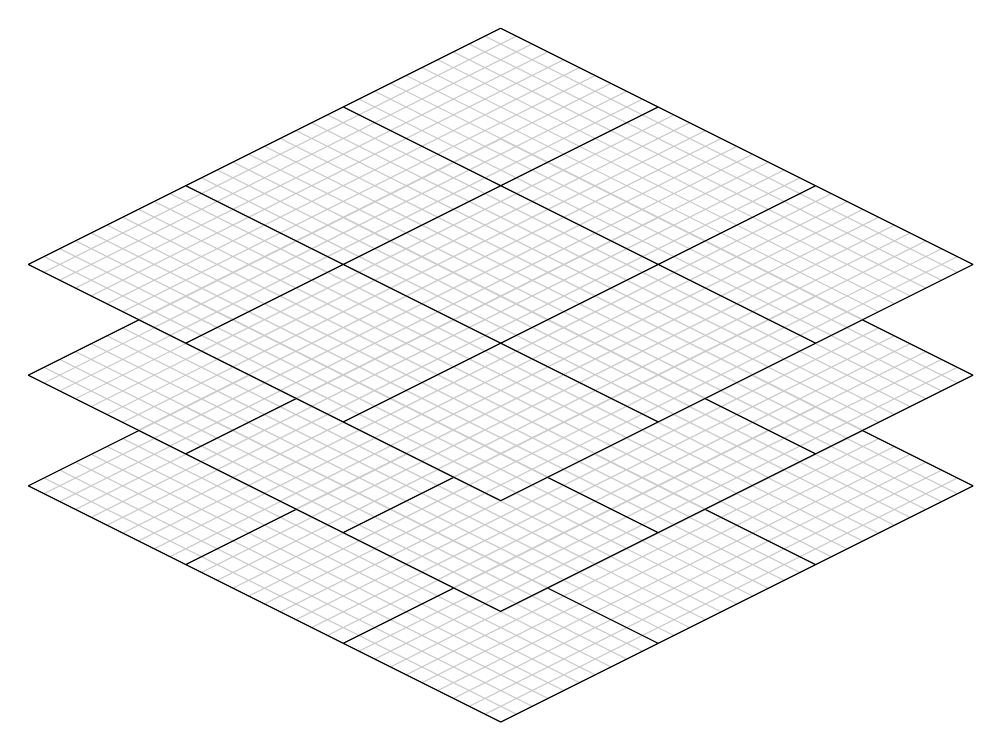
\begin{tikzpicture}[scale=2,every node/.style={minimum size=1cm},on grid]

	% Bottom of cube
	\begin{scope}[
			yshift=0,
			every node/.append style={
			yslant=0.5,xslant=-1},yslant=0.5,xslant=-1
		]
		\fill[white,fill opacity=0.8] (0,0) rectangle (3,3);
		\draw[step=1mm, black!20,thin] (0,0) grid (3,3);
		\draw[step=10mm, black] (0,0) grid (3,3);
	\end{scope}

	% Division
	\begin{scope}[
			yshift=20,
			every node/.append style={
			yslant=0.5,xslant=-1},yslant=0.5,xslant=-1
		]
		\fill[white,fill opacity=0.8] (0,0) rectangle (3,3);
		\draw[step=1mm, black!20,thin] (0,0) grid (3,3);
		\draw[step=10mm, black] (0,0) grid (3,3);
	\end{scope}



	% Mid layer
	\begin{scope}[
			yshift=40,
			every node/.append style={
			yslant=0.5,xslant=-1},yslant=0.5,xslant=-1
		]
		\fill[white,fill opacity=0.8] (0,0) rectangle (3,3);
		\draw[step=1mm, black!20,thin] (0,0) grid (3,3);
		\draw[step=10mm, black] (0,0) grid (3,3);
	\end{scope}


\end{tikzpicture}

\newpage

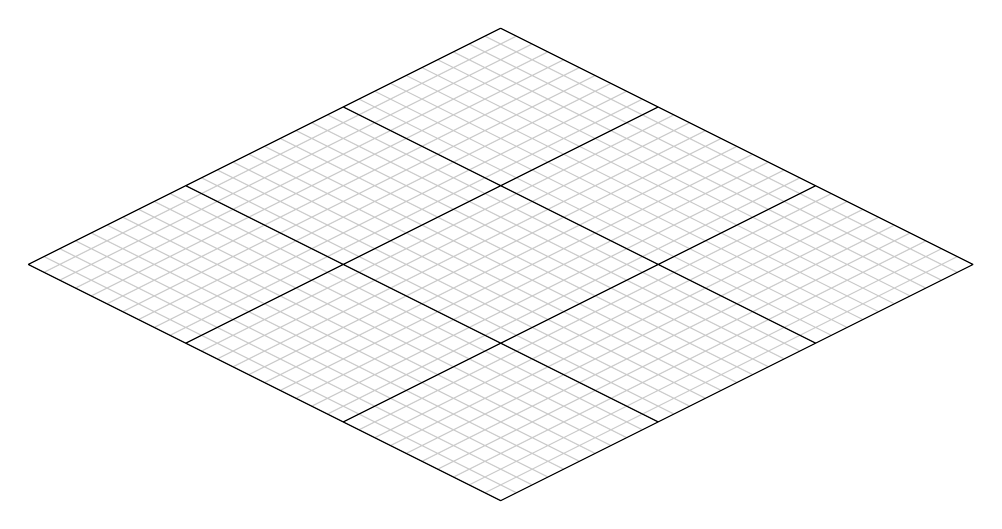
\begin{tikzpicture}[scale=2,every node/.style={minimum size=1cm},on grid]
	% Bottom of cube
	\begin{scope}[
			yshift=0,every node/.append style={
			yslant=0.5,xslant=-1},yslant=0.5,xslant=-1
		]
		\fill[white,fill opacity=0.9] (0,0) rectangle (3,3);
		\draw[step=1mm, black!20,thin] (0,0) grid (3,3);
		\draw[step=10mm, black] (0,0) grid (3,3);
	\end{scope}
\end{tikzpicture}

\newpage

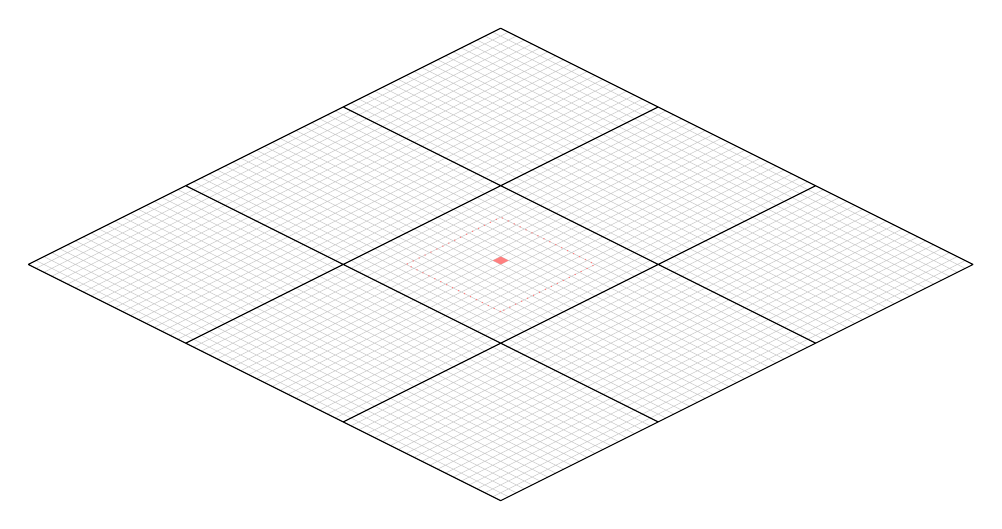
\begin{tikzpicture}[scale=2,every node/.style={minimum size=1cm},on grid]
	% Bottom of cube
	\begin{scope}[every node/.append style={yslant=0.5,xslant=-1},yslant=0.5,xslant=-1 ]
		\draw[step=0.5mm, black!20,very thin] (0,0) grid (3,3);
		\draw[step=10mm, black] (0,0) grid (3,3);
		\draw[red!50,dotted] (1.2,1.2) rectangle (1.8,1.8);
	  \fill[red!50] (1.50,1.50) rectangle (1.55,1.55);
	\end{scope}
\end{tikzpicture}

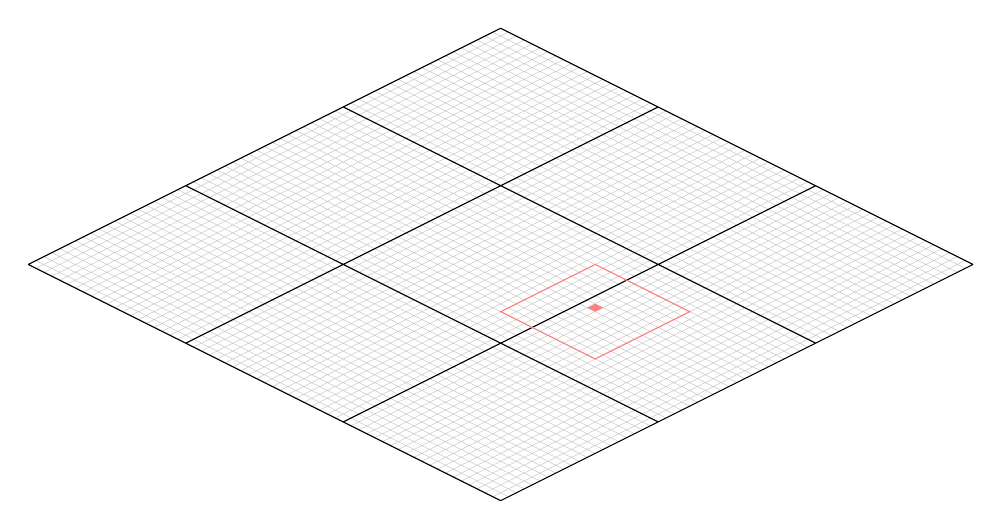
\begin{tikzpicture}[scale=2,every node/.style={minimum size=1cm},on grid]
	% Bottom of cube
	\begin{scope}[every node/.append style={yslant=0.5,xslant=-1},yslant=0.5,xslant=-1 ]
		\draw[step=0.5mm, black!20,very thin] (0,0) grid (3,3);
		\draw[step=10mm, black] (0,0) grid (3,3);
		\draw[red!50,thin] (1.2,1.2) rectangle (1.8,0.6);
		\fill[red!50] (1.50,0.9) rectangle (1.55,0.95);
	\end{scope}
\end{tikzpicture}

\newpage

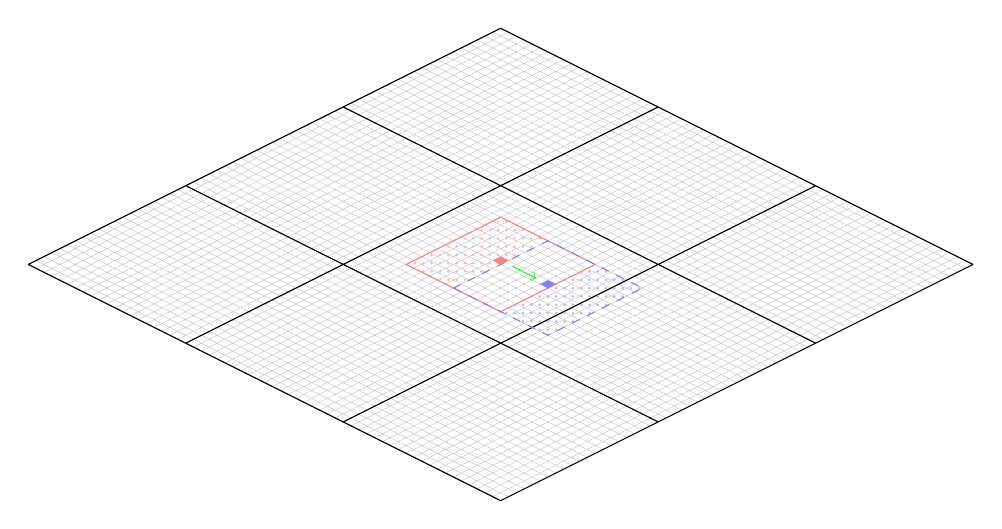
\begin{tikzpicture}[scale=2,every node/.style={minimum size=1cm},on grid]
	% Bottom of cube
	\begin{scope}[every node/.append style={yslant=0.5,xslant=-1},yslant=0.5,xslant=-1 ]
		\draw[step=0.5mm, black!20,very thin] (0,0) grid (3,3);
		\draw[step=10mm, black] (0,0) grid (3,3);



	  \fill[pattern=dots, pattern color=red!30] (1.2,1.5) rectangle (1.8,1.8);
		\fill[pattern=dots, pattern color=blue!30] (1.2,1.2) rectangle (1.8,0.9);

		\draw[red!50] (1.2,1.2) rectangle (1.8,1.8);
		\draw[blue!50,dashed] (1.2,1.5) rectangle (1.8,0.9);

	  \fill[red!50] (1.50,1.50) rectangle (1.55,1.55);
		\fill[blue!50] (1.50,1.2) rectangle (1.55,1.25);

		\draw[->,out=-45, in=45, looseness=0.9, green!90] (1.525,1.45) -- (1.525,1.3);
		% \node (node) at (0,0) {0};
		% \node (node) at (3,0) {x};
		% \node (node) at (0,3) {y};
		% \node (node) at (3,3) {3,3};
		% \node (node) at (1.8,0.6) {1.8,0.6};
		% \node (node) at (1.2,1.2) {1.2,1.2};

	\end{scope}
\end{tikzpicture}

\newpage


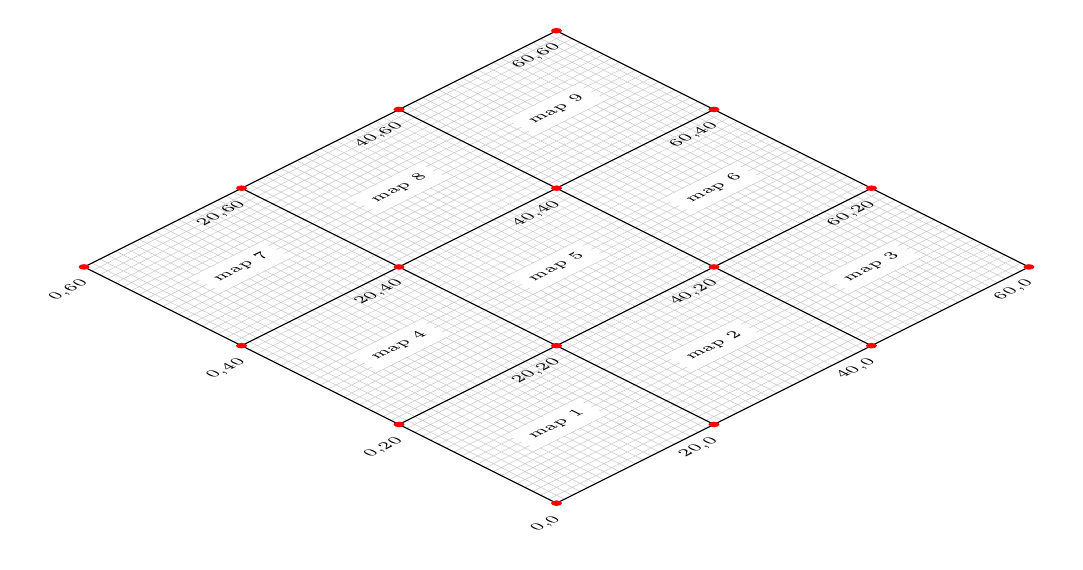
\begin{tikzpicture}[scale=2,on grid, label distance=0.01mm]
	% Bottom of cube
	\begin{scope}[every node/.append style={yslant=0.5,xslant=-1},yslant=0.5,xslant=-1 ]
		\draw[step=0.5mm, black!20,very thin] (0,0) grid (3,3);
		\draw[step=10mm, black] (0,0) grid (3,3);


  	\node [shape=circle,fill=red,label=left:{\tiny 0,0}, scale=0.3] (node) at (0,0) {};
		\node [shape=circle,fill=red,label=left:{\tiny 20,0},scale=0.3] (node) at (1,0) {};
		\node [shape=circle,fill=red,label=left:{\tiny 40,0},scale=0.3] (node) at (2,0) {};
		\node [shape=circle,fill=red,label=left:{\tiny 60,0},scale=0.3] (node) at (3,0) {};

		\node [shape=circle,fill=red,label=left:{\tiny 0,20},scale=0.3] (node) at (0,1) {};
		\node [shape=circle,fill=red,label=left:{\tiny 20,20},scale=0.3] (node) at (1,1) {};
		\node [shape=circle,fill=red,label=left:{\tiny 40,20},scale=0.3] (node) at (2,1) {};
		\node [shape=circle,fill=red,label=left:{\tiny 60,20},scale=0.3] (node) at (3,1) {};

		\node [shape=circle,fill=red,label=left:{\tiny 0,40},scale=0.3] (node) at (0,2) {};
		\node [shape=circle,fill=red,label=left:{\tiny 20,40},scale=0.3] (node) at (1,2) {};
		\node [shape=circle,fill=red,label=left:{\tiny 40,40},scale=0.3] (node) at (2,2) {};
		\node [shape=circle,fill=red,label=left:{\tiny 60,40},scale=0.3] (node) at (3,2) {};

		\node [shape=circle,fill=red,label=left:{\tiny 0,60},scale=0.3] (node) at (0,3) {};
		\node [shape=circle,fill=red,label=left:{\tiny 20,60},scale=0.3] (node) at (1,3) {};
		\node [shape=circle,fill=red,label=left:{\tiny 40,60},scale=0.3] (node) at (2,3) {};
		\node [shape=circle,fill=red,label=left:{\tiny 60,60},scale=0.3] (node) at (3,3) {};

		\node [shape=rectangle, fill=white!10] (text) at (.5,.5) {\tiny map 1};
		\node [shape=rectangle, fill=white!90] (text) at (1.5,.5) {\tiny map 2};
		\node [shape=rectangle, fill=white] (text) at (2.5,.5) {\tiny map 3};

		\node [shape=rectangle, fill=white] (text) at (.5, 1.5) {\tiny map 4};
		\node [shape=rectangle, fill=white] (text) at (1.5,1.5) {\tiny map 5};
		\node [shape=rectangle, fill=white] (text) at (2.5,1.5) {\tiny map 6};

		\node [shape=rectangle, fill=white] (text) at (.5, 2.5) {\tiny map 7};
		\node [shape=rectangle, fill=white] (text) at (1.5,2.5) {\tiny map 8};
		\node [shape=rectangle, fill=white] (text) at (2.5,2.5) {\tiny map 9};

	\end{scope}
\end{tikzpicture}
\end{document} 
